\documentclass[12pt]{report}
\usepackage[a4paper, width=150mm,top=25mm,bottom=25mm]{geometry}
\usepackage[utf8]{inputenc}
\usepackage{blindtext}
\usepackage{graphicx}
\usepackage{lipsum}
\usepackage{times}
\usepackage{titlesec}
\usepackage{tocloft}
\usepackage{pdfpages}
\usepackage{amsmath}
\usepackage{listings}
\usepackage{xcolor}
\usepackage{tikz}
\usepackage{pgf-umlcd}
\usepackage{caption}
\usepackage{subcaption}
\usepackage[colorlinks=true,linkcolor=black,urlcolor=black,citecolor=black]{hyperref}
\usetikzlibrary{positioning, shapes.geometric, arrows,calc,arrows.meta}
\graphicspath{{images/}}

% Define block styles
\tikzstyle{block} = [rectangle, draw, fill=blue!20, 
    text width=5em, text centered, rounded corners, minimum height=4em]
\tikzstyle{sum} = [draw, fill=blue!20, circle, minimum size=1cm, node distance=1.5cm]
\tikzstyle{input} = [coordinate]
\tikzstyle{output} = [coordinate]
\tikzstyle{pidblock} = [draw, dashed, inner sep=0.5cm, rounded corners]

% Define custom colors
\definecolor{mygreen}{rgb}{0,0.6,0}
\definecolor{mygray}{rgb}{0.5,0.5,0.5}
\definecolor{mymauve}{rgb}{0.58,0,0.82}
\definecolor{backcolour}{rgb}{0.95,0.95,0.92}

% Set up listings for MATLAB, Python, and C
\lstset{ 
    backgroundcolor=\color{backcolour},   % choose the background color
    basicstyle=\ttfamily\footnotesize,  % the size of the fonts that are used for the code
    breakatwhitespace=false,         % sets if automatic breaks should only happen at whitespace
    breaklines=true,                 % sets automatic line breaking
    captionpos=b,                    % sets the caption-position to bottom
    frame=single,                    % adds a frame around the code
    keepspaces=true,                 % keeps spaces in text, useful for keeping indentation
    numbers=left,                    % where to put the line-numbers
    numbersep=5pt,                   % how far the line-numbers are from the code
    numberstyle=\tiny\color{mygray}, % the style that is used for the line-numbers
    rulecolor=\color{black},         % if not set, the frame-color may be changed on line-breaks within not-black text (e.g. comments (green here))
    showspaces=false,                % show spaces adding particular underscores
    showstringspaces=false,          % underline spaces within strings
    showtabs=false,                  % show tabs within strings adding particular underscores
    tabsize=2,                       % sets default tabsize to 2 spaces
    title=\lstname                   % show the filename of files included with \lstinputlisting; also try caption instead of title
}

% MATLAB settings
\lstdefinestyle{MATLAB}{
    language=Matlab,
    keywordstyle=\color{blue},
    commentstyle=\color{mygreen},
    stringstyle=\color{mymauve}
}

% Python settings
\lstdefinestyle{Python}{
    language=Python,
    keywordstyle=\color{blue},
    commentstyle=\color{mygreen},
    stringstyle=\color{mymauve}
}

% C settings
\lstdefinestyle{C}{
    language=C,
    keywordstyle=\color{blue},
    commentstyle=\color{mygreen},
    stringstyle=\color{mymauve}
}

\renewcommand{\cftchapleader}{\cftdotfill{\cftdotsep}} 
\renewcommand{\cftchapfont}{\normalfont\bfseries}

\newcommand{\name}{Shashank Agarwal}
\newcommand{\faculty}{Dr.Loveleen Kaur Taneja}
\newcommand{\industry}{Mr.Sarv Parteek Singh}
\newcommand{\director}{Mr.M.S. Saini}

\begin{document}

\begin{titlepage}
    \begin{center}
        \vspace*{-3cm}
        
\includegraphics{university.png}\\
        {\huge\textbf{Project Report}}\\

        \vspace*{1cm}
        {\Large Design of Front end converter using SVPWM technique}

        \vfill
        Submitted by

        \vfill
        Shashank Agarwal\\
        21104027

        \vfill
        Under the Guidance of
    \end{center}
    \vfill

    \noindent
    \begin{minipage}[t]{0.45\textwidth}
        Mr. Sarv Prateek Singh\\
        Technical Advisor\\
        Statcon Electronics Pvt Ltd\\
        Noida
    \end{minipage}
    \hfill
    \begin{minipage}[t]{0.45\textwidth}
        \raggedleft
        Dr. Tejinder Singh Saggu\\
        Faculty Coordinator\\
        Punjab Engineering College\\
        (Deemed to be University)\\
        Chandigarh
    \end{minipage}
\end{titlepage}
\setlength{\parindent}{0pt}
\pagenumbering{roman}

\titleformat{\chapter}[display]
{\normalfont\huge\bfseries\centering}{\thechapter.}{20pt}{\Large}

\chapter*{Declaration}
I hereby declare that the project work entitled "Design of Active Front End" is
an authentic record of my own work carried out at Statcon Electronics India Ltd
as requirements of six months project semester for the award of degree of
B.E./B.Tech. Electrical Engineering, Punjab Engineering College (Deemed to be
University), Chandigarh, under the guidance of Mr. Sarv Parteek Singh and Dr.
Tejinder Singh Saggu, during January to June, 2024.

\vspace*{2.5cm}
\noindent
\begin{minipage}[t]{0.5\textwidth}
    \raggedright
    {Date: {\today}}
\end{minipage}
\hfill
\begin{minipage}[t]{0.5\textwidth}
    \raggedleft
    {Shashank Agarwal\\
    21104027}

\end{minipage}
\vfill

\noindent
Certified that the above statement made by the student is correct to the best of our knowledge and belief.

\vspace*{2cm}

\noindent
\begin{minipage}[t]{0.5\textwidth}
    \raggedright
    Dr. Tejinder Singh Saggu\\
    Faculty Coordinator\\
    Department of Electical Engineering\\
    Punjab Engineering College (Deemed to be University),\\
    Chandigarh
\end{minipage}
\hfill
\begin{minipage}[t]{0.5\textwidth}
    \raggedleft
    Mr. Sarv Parteek Singh\\
    Technical Advisor\\
    Statcon Electronics India Ltd,\\
    Noida

\end{minipage}

\chapter*{Acknowledgement}
\input{chapters/acknowledgement}

\titleformat{\chapter}[hang]
{\normalfont\LARGE\bfseries}{\thechapter.}{20pt}{\LARGE}

\tableofcontents
\listoffigures

\clearpage
\pagenumbering{arabic}

\chapter{Summary}
I got the opportunity to do my internship at Statcon Electronics India Ltd.
Statcon Electronics established in 1986 is one of India's largest ISO
9001-20151 certified manufacturer of Static energy Conversion system. During my
internship at Satcon Electronics India Ltd, Noida, I was first assigned to
explore Space Vector Modulation technique and then make a simulation for a
front end converter using Space Vector Modulation. I was part of the Embedded
Software team and my task was to develop a control algorith for the front end
converter.\\

The aim of the project to design a Active Front End converter for a Hybrid
inverter,aiming to enhance its efficiency and performance while reducing
harmonic distortions and improving the power factor.

\section{Timeline}
My internship at Statcon Electronics India Ltd started on 10th January, 2024.
My mentor gave me the task of exploring Space Vector Modulation and developing
control algorithm for the front end converter. This timeline will briefly
explain the course of my internship from beginning to end.

\subsection{January}
In January, I started learning about Space Vector Pulse Width Modulation
(SVPWM). This involved understanding two important things: the Clarke and Park
transforms. These transforms help to change three-phase voltages into a simpler
two-dimensional form, making it easier to control three-phase systems. The
Clarke transform turns three-phase voltages into two-phase parts, while the
Park transform changes these parts into a fixed frame of reference. I also
learned about space vectors, which show how the three-phase voltages combine.
This knowledge helped me understand SVPWM better. It's a technique that uses
space vectors to control how inverters produce voltage. This exploration gave
me a better grasp of how SVPWM works and its uses in power electronics.

\subsection{Feburary}
During February, I immersed myself in the study of the Clarke and Park
transforms, essential mathematical tools used in analyzing three-phase
electrical systems.The Clarke transform simplifies three-phase voltages into
two-phase components, making it easier to understand and analyze complex
electrical systems. Similarly, the Park transform further refines these
components into a fixed frame of reference, streamlining the analysis and
control of electrical signals. Alongside theoretical exploration, I practically
experimented by developing Python code to implement and test these
transformations. This hands-on approach not only deepened my understanding of
the transforms but also provided valuable insights into their real-world
applications and implementation challenges.

\subsection{March}

During March, I worked on developing and testing a three-phase Phase-Locked
Loop (PLL) algorithm using Python. This algorithm used the Clarke and Park
transforms to precisely estimate the angle of the space vector in the
three-phase system. Following the initial testing phase of the PLL algorithm in
Python, I transitioned to Simulink/MATLAB for further simulation. Within the
Simulink environment, I used MATLAB function blocks to implement the PLL
algorithm. Once this was completed, I proceeded to make a three-phase inverter
in Simulink using IGBT components. Leveraging MATLAB function blocks and the
output of the PLL, I then generated gate timing signals for the Front end of
the inverter, ensuring precise control and synchronization of the electrical
signals.

\subsection{April}

In April, I worked toward fine-tuning the Proportional-Integral (PI) controller
for the Phase-Locked Loop (PLL) using the Ziegler–Nichols method. This involved
adjusting the parameters of the PI controller to optimize the performance of
the PLL algorithm. By employing the Ziegler–Nichols method, I aimed to achieve
stability and responsiveness in tracking and synchronizing the phase of
electrical signals effectively. Additionally, I implemented a control loop in
MATLAB function blocks to measure the current flowing from the front end to the
grid. This control loop allowed for the adjustment of the output voltage to
either draw or supply the desired current, depending on the system
requirements.

\subsection{May}
\blindtext

\subsection{June}
\blindtext
\chapter{Introduction}
An active front-end (AFE) converter, is a grid interface converter that
transfers power between an energy source and the utility grid, and between the
utility grid and a load. It's a controllable rectifier that can exchange power
between AC and DC power in both directions, and can regenerate power to the
mains to reduce power costs.
\section{Problem Statement}
My team at Statcon Electronics India Ltd has been focusing on on enhancing the
efficiency and performance of front-end converters. Presently, most active
front-end converters utilize Silicon Controlled Rectifiers (SCRs) for
rectification, employing a conventional 6-pulse converter configuration. My
task was to explore and design a active front-end using Insulated Gate Bipolar
Transistors (IGBTs) as alternatives to SCRs in the rectification process.\\

The primary objective of this project is to investigate the feasibility and
advantages of using IGBTs instead of SCRs for rectification in active front-end
converters. Specifically, we aim to implement a Space Vector Pulse Width
Modulation (SVPWM) technique to control the IGBTs effectively. This technique
offers precise control over the switching patterns of the IGBTs, allowing for
optimized power conversion and reduced harmonic distortion.\\

Furthermore, the project involves the development of a sophisticated control
algorithm to manage the operation of the IGBTs. This algorithm must facilitate
seamless transition between pulling current from the grid (rectification mode)
and supplying current to the grid (regeneration mode). The control system
should ensure stable and efficient operation under varying load conditions
while maintaining compliance with grid standards and regulations.

\section{Overview}
A three-phase AC to DC converter is essential for many power electronics system
such as Variable frequency drive (VFD), battery charger, uninterruptible power
supplies (UPS).

Traditionally diode rectifiers or thyristor rectifier are used for AC to DC
conversion, both these rectifiers behave as non- linear loads. The currents
drawn by the rectifiers include a fundamental component and harmonic
components. The voltage drop across the line inductance due to the harmonic
currents distorts the mains voltage. Consequently, the other loads connected to
the mains are also fed with a distorted voltage.

\subsection{Traditional Rectifier}
Diode rectifier, depicted in Figure~\ref{fig:diode_rectifier}, produces a
constant DC voltage, which is a function of the system voltage. A thyristor
based rectifier can produce a variable DC voltage. But, both these topology
behave as non-linear loads.

\begin{figure}[h]
    \centering
    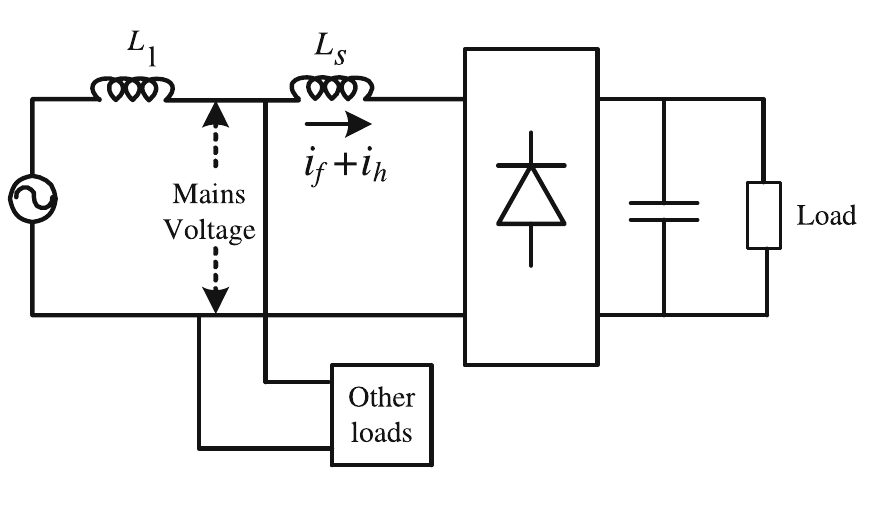
\includegraphics[width=\textwidth]{Diode Rectifier.png}
    \caption{AC to DC Conversion using Diode Rectifier.}
    \label{fig:diode_rectifier}
\end{figure}

\subsection{IGBT Rectifier}
\begin{figure}[h]
    \centering
    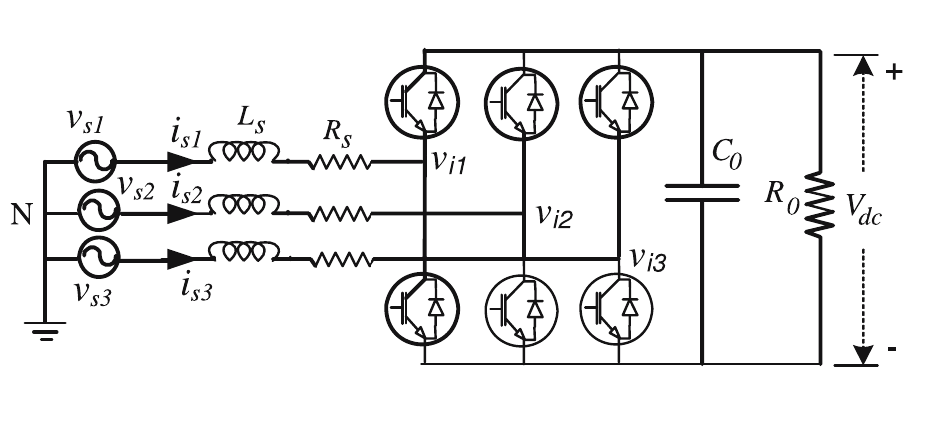
\includegraphics[width=\textwidth]{IGBT Rectifer.png}
    \caption{Schematic diagram of
        a front-end converter (FEC)}
    \label{fig:igbt_rectifier}
\end{figure}
\noindent
IGBT Rectifer, depicted in Figure~\ref{fig:igbt_rectifier}, draws near
sinusoidal current from grid. The power factor as well as DC Voltage can be
adjusted. Since it is connected to line side it is called line side or front
end converter.

The converter consists of a three-phase bridge, a high capacitance on the dc
side and a three-phase inductor in the line-side. The voltage at the mid point,
$V_i$ is pulse width modulated (PWM) in nature. The voltage consists of a
fundamental component (at line frequency) besides harmonic components around
the switching frequency of the converter. Being at high frequencies, these
harmonic components are well filtered by the line inductor. Hence the current
is near sinusoidal. The fundamental component of $V_i$ controls the flow of
real and reactive power.

\subsection{Vector Control}
Vector control is a popular method for control of three-phase induction motors.
The basic idea of this scheme is to control the flux producing and the
torque-producing components of motor current. The outer control loop controls
the speed of the motor, while the inner loop controls the components of current
vector, which correspond to torque and flux. Similar control approach can be
used for FEC also. Here, the three-phase grid voltages and line currents are
converted into an equivalent two-phase system, called stationary reference
frame . These quantities are further transformed into
a reference frame called synchronous reference frame, which revolves at the
grid frequency .

\subsection{Space Vector Modulation}
This technique, also known as Space Vector Pulse Width Modulation (SVPWM), is a
method used to generate the switching signals for the IGBTs in the AFE
converter. It offers precise control over the IGBT switching patterns by
synthesizing the desired output voltage as a combination of multiple voltage
vectors. SVM has eight space vectors, other space vectors are synthesized by
alternating active and zero vectors over a switching period.

\section{Challenges}
I faced many challenges in developing a Active front-end converter. Firstly,
distinguishing between Sinusoidal Pulse Width Modulation (SPWM) and Space
Vector Pulse Width Modulation (SVPWM) posed confusion due to their perceived
similarity in operational principles. Secondly, reconciling the non-zero
resultant vector in SVPWM with the traditional understanding of three-phase
systems, where the vector sum equals zero, required conceptual clarification to
ensure accurate system design and analysis. Another challenge was comprehending
how rectification and regeneration can occur through the same IGBT bridge, as
it involved bidirectional power flow management. Additionally, not knowing how
to write code in MATLAB was another challenge, but learning it opened up new
possibilities for simulating and analyzing our AFE converter designs.
\chapter{Work}
\section{Simulation}
\begin{figure}[h]
    \centering
    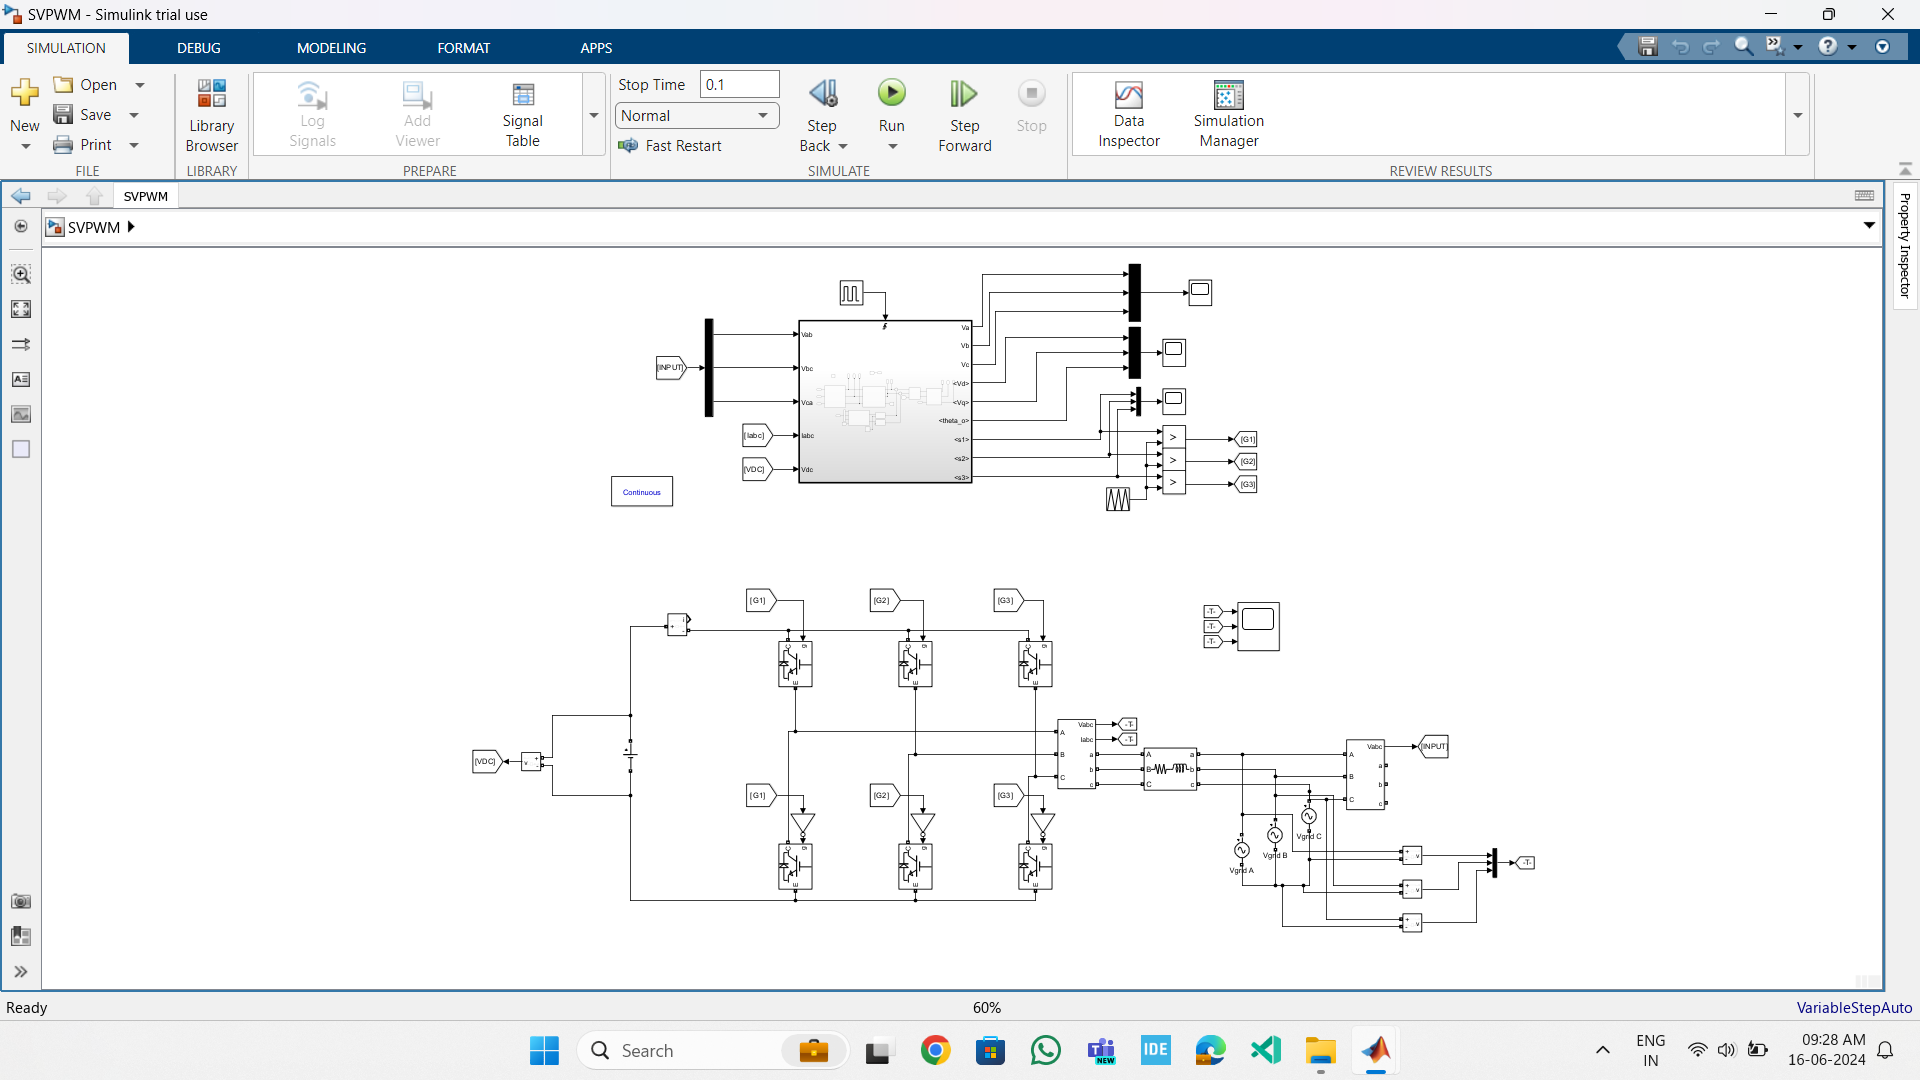
\includegraphics[width=\textwidth]{Whole Simulation.png}
    \caption{Simulation}
    \label{fig:Simulation}
\end{figure}
Before initiating the implementation phase, it was imperative to conduct a
comprehensive simulation of the front end using Simulink/MATLAB. The simulation
setup involved importing a three-phase source from MATLAB and configuring the
necessary parameters for voltage and current measurements.

\subsection{MATLAB Function Blocks in Simulation}
To emulate the behavior of a microcontroller in the simulation environment,
MATLAB function blocks were extensively utilized. These function blocks
provided a familiar coding environment, resembling the programming paradigms
employed in microcontroller firmware development. By encapsulating custom
algorithms and control logic within MATLAB function blocks, it was possible to
simulate complex control strategies and signal processing techniques with ease.
This approach not only facilitated rapid prototyping and testing but also
provided invaluable insights into the real-time behavior of the system. The use
of MATLAB function blocks bridged the gap between simulation and
implementation, enabling seamless transition from design validation to hardware
deployment.
\subsection{Control System}
\begin{figure}[h]
    \centering
    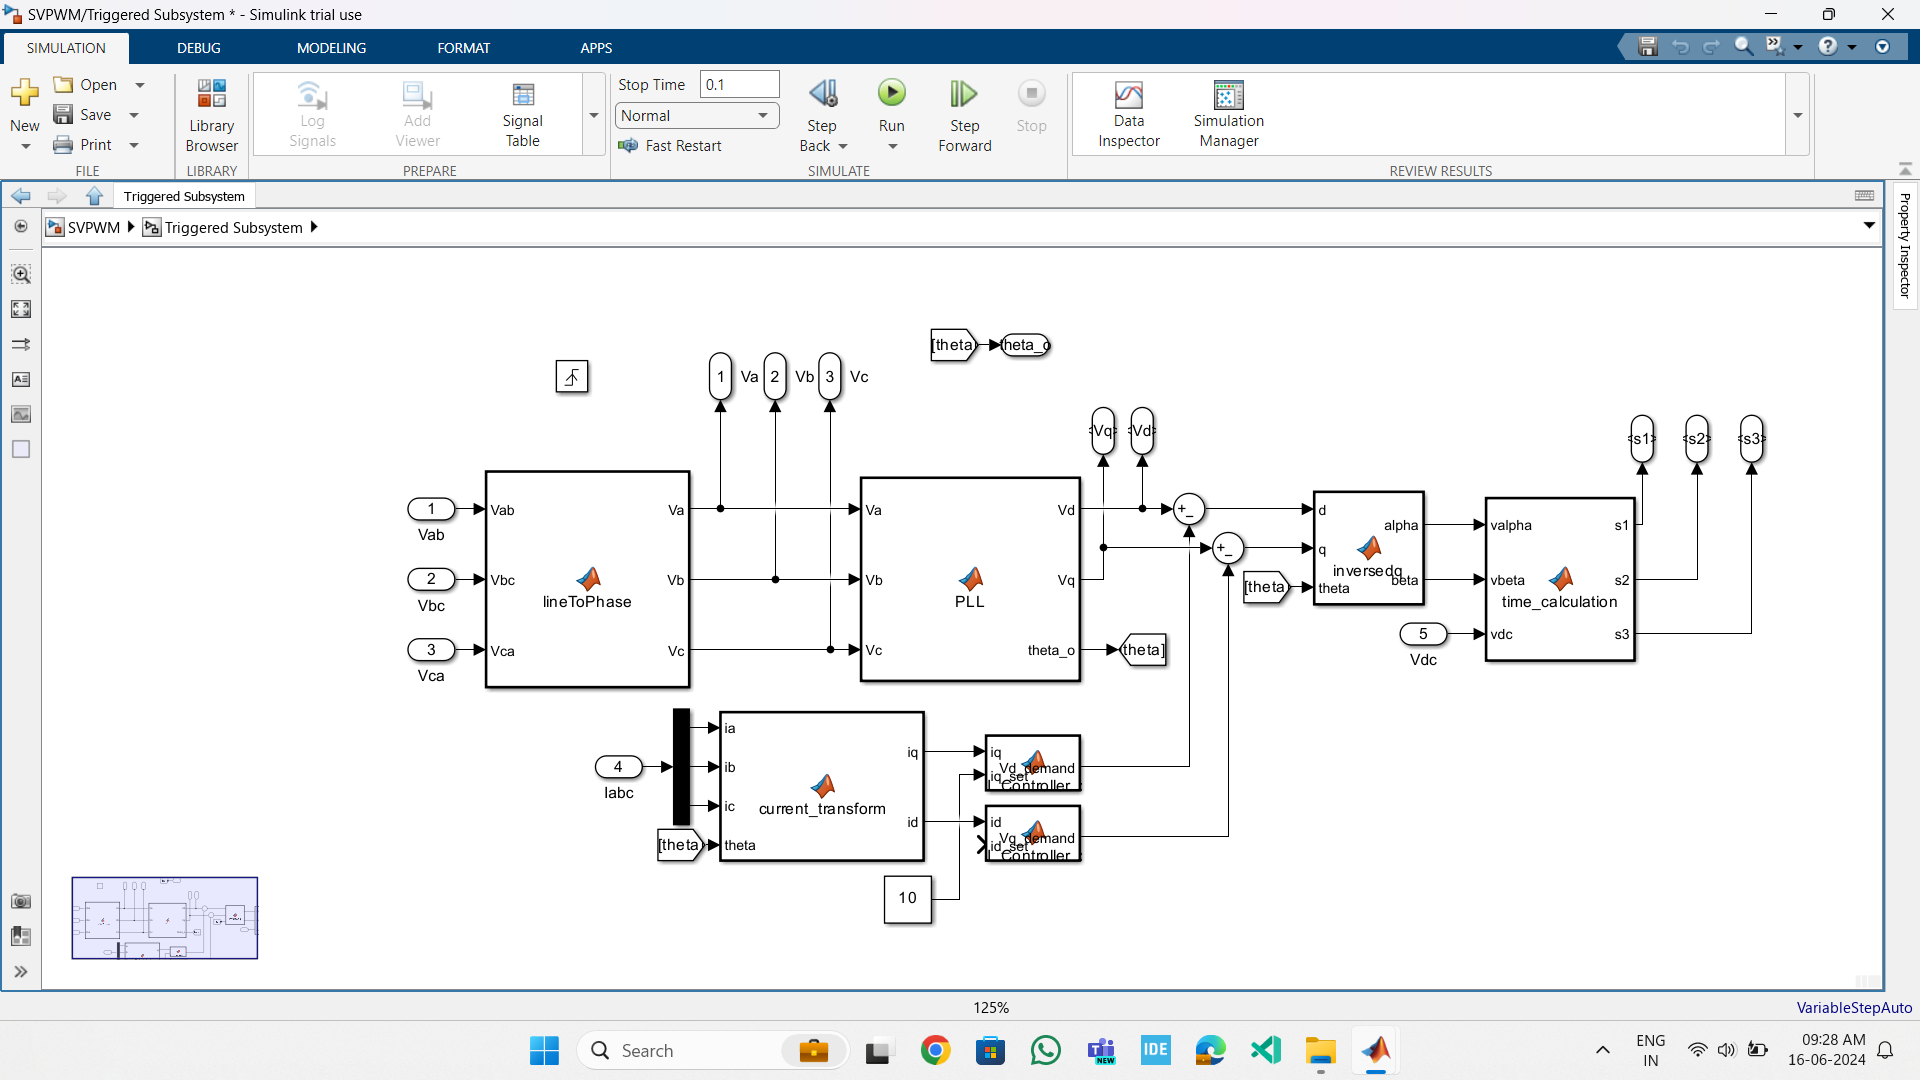
\includegraphics[width=\textwidth]{Control flow.png}
    \caption{Control System}
    \label{fig:Control System}
\end{figure}
\subsubsection{Voltage Transformation}
Transform the measured line voltages from the three-phase source into the
alpha-beta frame using the Clarke transform. This transformation facilitates
easier analysis and control of the three-phase system. The Clarke transform
converts three-phase voltages into two orthogonal components (alpha and beta),
simplifying the analysis of the system's dynamics and making it easier to
implement control strategies.

\subsubsection{Phase-Locked Loop (PLL)}
Incorporate a Phase-Locked Loop (PLL) block to convert the voltages from the
alpha-beta frame to the dq rotating reference frame. Additionally, the PLL
provides the angle theta of the voltage vector, crucial for subsequent control
strategies. The PLL ensures synchronization with the grid by maintaining a
constant phase relationship, which is vital for accurate control and stability
of the system.

\subsubsection{Current Measurement and Transformation}
Measure the line current flowing into the front end, and using Clarke and Park
transform blocks, convert it to the dq reference frame. Utilize the angle theta
obtained from the PLL for this transformation. The dq reference frame allows
for decoupled control of the direct and quadrature components of the current,
enabling more precise control of the active and reactive power.

\subsubsection{Current Regulation}
Regulate the current flowing into the front end to ensure stable operation and
adherence to system constraints. Employ two Proportional-Integral (PI)
controllers to compare the measured current to a predetermined set current
value and generate control signals for current regulation. The PI controllers
adjust the control signals to minimize the error between the measured and
desired current values, ensuring the system operates within the desired
parameters.

\subsubsection{Voltage Calculation and Transformation}
Add the control signals (delta Vq and delta Vd) obtained from the PI
controllers to the Vq and Vd components obtained from the PLL. Convert these
voltages back to the Clarke frame using the inverse Park transform. This step
integrates the control efforts with the system's voltages, transforming the
controlled voltages back into the stationary reference frame for further
processing and application.

\subsubsection{Gate Timing Calculation}
Utilize the voltages calculated in the previous step (V alpha* and V beta*) to
determine gate timings for the three-phase active front end. These gate timings
dictate the switching patterns of the Insulated Gate Bipolar Transistors
(IGBTs), essential for controlling the flow of current through the front end.
The precise timing of the IGBT switching is crucial for maintaining the desired
current and voltage waveforms, ensuring efficient and stable operation of the
power conversion system.

\subsection{Power System}
\begin{figure}[h]
    \centering
    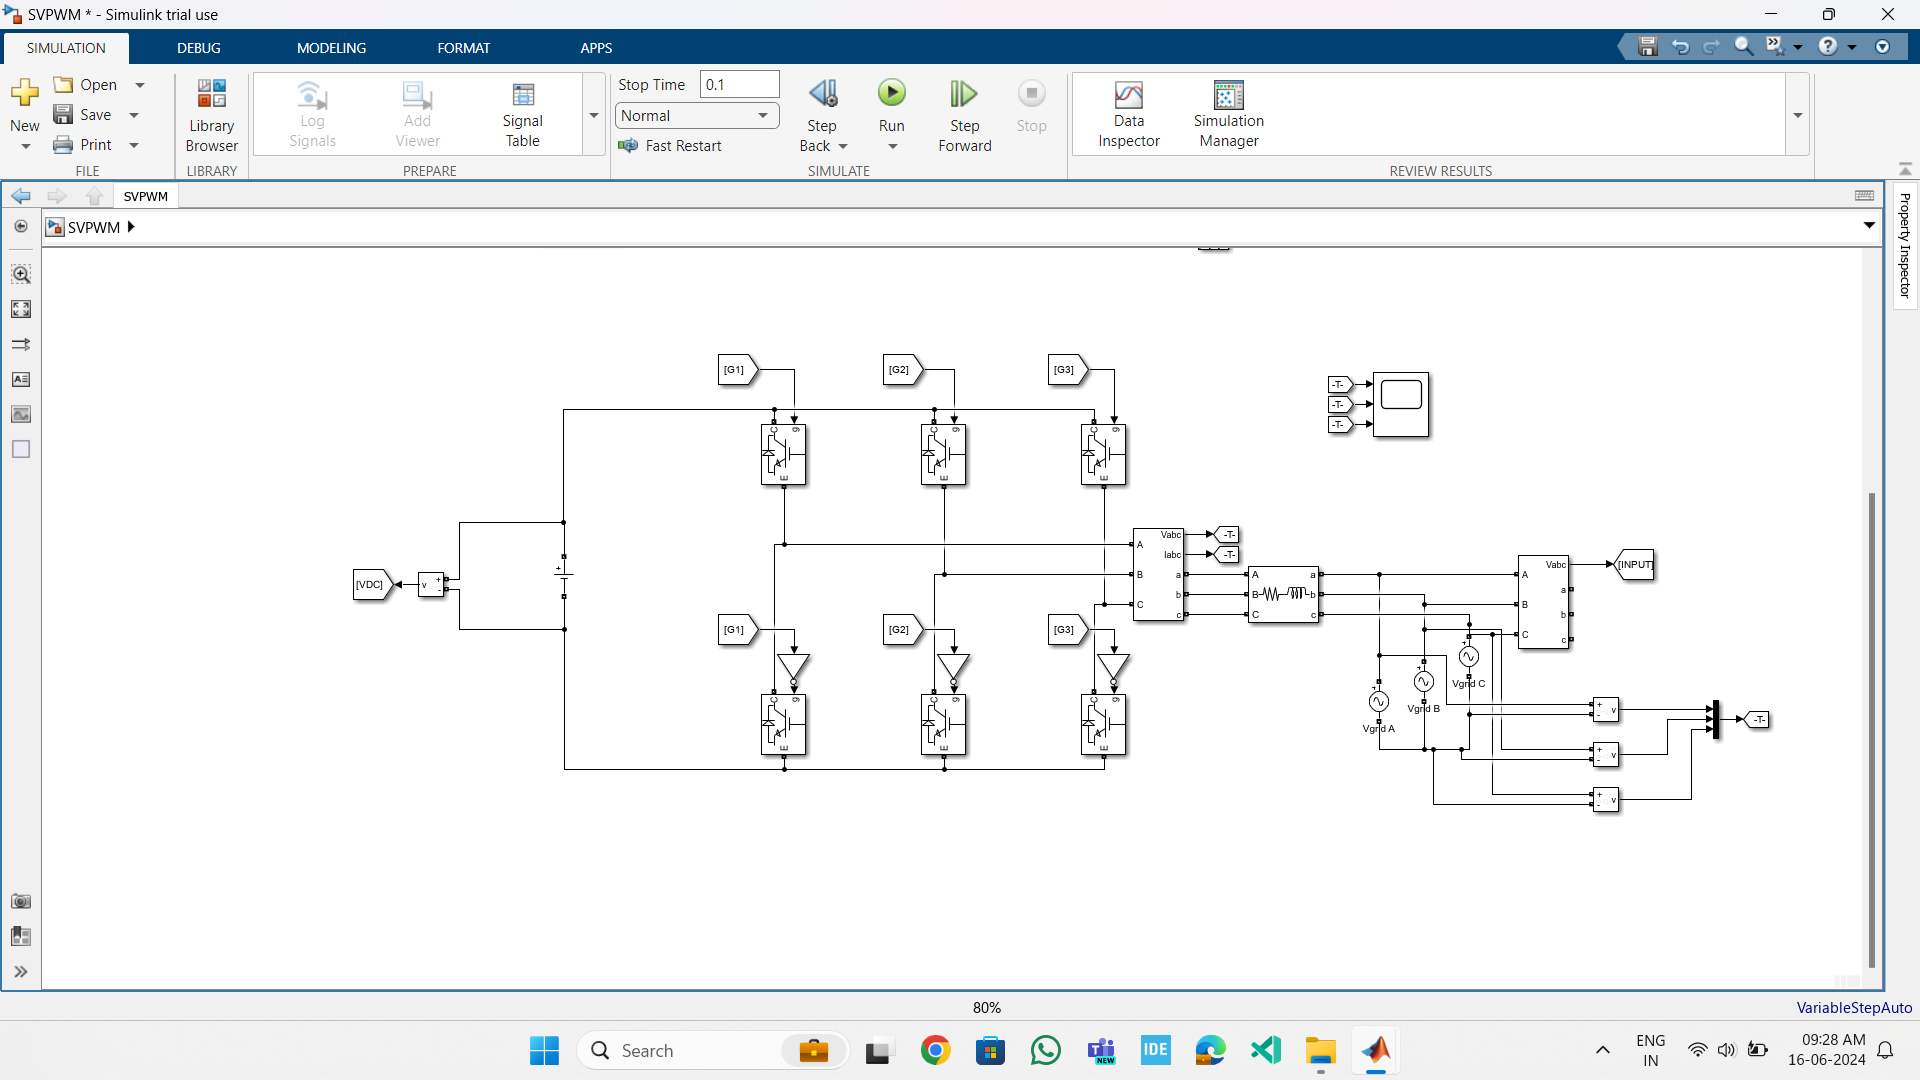
\includegraphics[width=\textwidth]{Power System.png}
    \caption{Power System}
    \label{fig:Power System}
\end{figure}

\subsubsection{Three-Phase AC Source}
The Three-Phase AC Source serves as the input power to the system.It provides
three sinusoidal voltage waveforms with a 120-degree phase difference between
each phase.The amplitude and frequency of the AC source are determined based on
the grid specifications or the application requirements.
\subsubsection{Three-Phase IGBT Bridge}
The Three-Phase IGBT Bridge is the primary power conversion and control element
in the system. It consists of six Insulated Gate Bipolar Transistors (IGBTs)
arranged in a three-phase bridge configuration. The IGBTs are switched in a
complementary manner to modulate the voltage across the load.

The IGBT bridge controls the flow of current from the AC source to the load by
switching the IGBTs on and off at precise intervals. This switching action
enables the conversion of AC power from the source to DC power, which can be
further conditioned or inverted as per the requirements of the application.

Additionally, the gate timing signals for the IGBTs are generated based on the
control signals calculated by the control system. These gate timing signals
dictate the switching pattern of the IGBTs, ensuring the desired current and
voltage waveforms are maintained for efficient and stable operation of the
power conversion system.

\section{Implementation}
\begin{figure}[h]
    \centering
    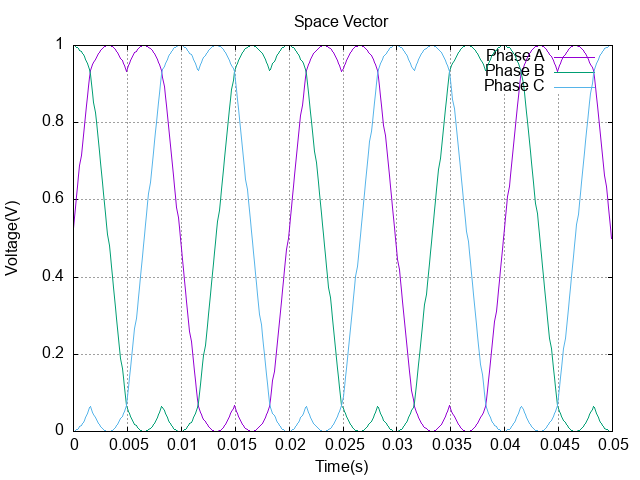
\includegraphics[width=\textwidth]{spacevector.png}
    \caption{Space Vector plotted using GNUPLOT}
    \label{fig:Space Vector Generated using C code}
\end{figure}
After completing the simulation using Simulink/MATLAB to validate
the system design and control strategies, the project transitioned to the
implementation stage on a microcontroller. This phase focused on translating
theoretical concepts into practical application. This section includes the
selection process of the microcontroller, development of essential
transformation functions in C, and the integration of hardware components such
as timers, Direct Memort Access (DMA), and Analog to Digital Converter (ADC)
for accurate system monitoring and control.

\subsection{Microcontroller Selection}
The first step in the implementation phase was choosing an appropriate
microcontroller for the project. After evaluating several options, the
STM32F411 was selected due to its Digital Signal Processing (DSP) and Floating
Point Unit (FPU) capabilities. These features allowed us to run the
Proportional-Integral-Derivative (PID) loop at a high frequency of 10kHz,
providing 200 samples per cycle. This high sampling rate was crucial for
achieving precise control and stability in the system.

\subsection{Implementation of Voltage transform functions}
To handle the transformations required for the control algorithms, I
implemented the Clarke and Park transform functions in C. The process began by
creating an array with synthetic values to simulate the inputs. These values
were then fed into the custom transformation functions. The output was verified
using GNUPLOT to ensure the accuracy of the transformations. This step was
essential to validate the mathematical operations and ensure the functions were
performing as expected.

\subsection{Microcontroller Programming and Testing}
With the transformation functions ready, I proceeded to program the STM32F411
microcontroller. This phase involved a deep dive into various aspects of the
microcontroller, including timers, Direct Memory Access (DMA), and
Analog-to-Digital Converters (ADC).
\begin{itemize}
    \item \textbf{ADC Sampling}: I utilized the ADC to sample the voltage values from the system. This real-time data acquisition was critical for the subsequent control processes.
    \item \textbf{Transformation and Modulation}: The sampled voltage values were processed using the previously developed Clarke and Park transform functions. This step generated the necessary parameters for Space Vector Modulation (SVM).
\end{itemize}
\noindent
The integration of these components allowed for the generation of space vector
modulated waves, essential for controlling the power conversion system
effectively. Each part of this process was meticulously tested to ensure
reliability and accuracy, laying a strong foundation for the successful
deployment of the control system.
\chapter{Details of work}
\section{Problem Statement}
\chapter{Conclusion and Future scope}
\section{Conclusion}
Throughout my internship at Statcon Electronics India Ltd., I gained extensive
knowledge and practical experience in implementing Space Vector Pulse Width
Modulation (SVPWM). This journey involved understanding and applying various
mathematical transformations, developing control algorithms, and transitioning
from simulation to real hardware implementation.

\noindent
SVPWM offers several advantages over conventional techniques, such as:
\begin{itemize}
    \item \textbf{Higher Efficiency}: SVPWM maximizes the DC bus voltage utilization, leading to improved efficiency in inverter operation. This is crucial for applications where energy efficiency is paramount, such as in renewable energy systems and electric vehicles.
    \item \textbf{Reduced Harmonic Distortion}: By optimizing the switching sequences, SVPWM reduces the harmonic distortion in the output waveforms. This results in cleaner and more stable power delivery, which is essential for sensitive electronic equipment and improving the overall power quality.
    \item \textbf{Improved Power Factor}: SVPWM enables better control over the output voltage and current, contributing to an improved power factor. This is beneficial in reducing energy losses and ensuring that power systems operate closer to their maximum efficiency.
\end{itemize}

\noindent
Moreover, the hands-on experience with simulation tools like MATLAB/Simulink
and practical implementation using STM32F411 microcontrollers has enriched my
understanding of both software and hardware aspects of power electronics. This
dual exposure has equipped me with a holistic view of the challenges and
solutions in modern inverter technology.

\section{Future Scope}
The knowledge and skills developed during this internship have broad
applications in various fields, including:

\begin{itemize}
    \item \textbf{Hybrid Inverters}: Enhancing the efficiency and performance of hybrid inverters. By integrating SVPWM, hybrid inverters can achieve better efficiency and reliability, making them more viable for both residential and commercial energy solutions.
    \item \textbf{Active Front Ends}: Driving DC series motors in trains for power factor correction and voltage regulation. Implementing SVPWM in active front-end converters can lead to significant improvements in power quality and energy savings in traction systems.
    \item \textbf{Battery Charging}: Implementing SVPWM for efficient battery charging systems. With the growing demand for electric vehicles and renewable energy storage, efficient battery charging solutions are critical. SVPWM can contribute to faster and more efficient charging cycles, prolonging battery life and enhancing performance.
    \item \textbf{Electric Vehicle (EV) Drive Systems}: Applying SVPWM in EV drive systems to improve motor efficiency and reduce energy consumption. This can lead to extended range and better performance of electric vehicles, making them more competitive with traditional internal combustion engine vehicles.
\end{itemize}

\noindent
Overall, this internship has been a valuable learning experience, providing me
with the technical expertise and practical skills needed to contribute
effectively to the field of power electronics and embedded systems. The
insights gained have not only broadened my knowledge base but also ignited a
passion for further exploration and innovation in this dynamic and impactful
field.
\begin{thebibliography}{9}
    \bibitem{clarke_transform}
Alpha–beta transformation. (2024, April 19). In Wikipedia. \url{https://en.wikipedia.org/wiki/Alpha%E2%80%93beta_transformation}.

\bibitem{DSP-Based Electromechanical Motion Control}
DSP-Based Electromechanical Motion Control. \url{httpas://kaliasgoldmedal.yolasite.com/resources/MCDSP/UNIT5/Clarke_park.pdf}

\bibitem{R. H. Park}R. H. Park, “Two-reaction theory of synchronous machines – Generalized method of analysis- Part I,” AIEE Trans., Vol. 48, July 1929, pp.716-727
\bibitem{E. Clarke}E. Clarke, Circuit Analysis of AC Power Systems, Vol. I- Symmetrical and Related Components, John Wiley and Sons, New York, 1943.

\end{thebibliography}

\end{document}
